\begin{figure}[h!]
\begin{center}
\scalebox{1.6}{
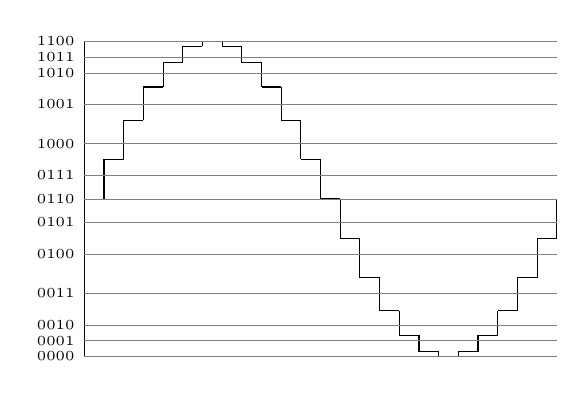
\begin{tikzpicture}
\shorthandoff{<>."}
  \draw[-] (0,-2) -- (0,2) node[right] {$$};
  \draw (0.25,0) -- (0.25,.5);
  \draw (0.25,.5) -- (0.5,.5);

  \draw (0.5,.5) -- (0.5,1);
  \draw (0.5,1) -- (0.75,1);

  \draw (0.75,01) -- (0.75,1.42);
  \draw (0.75,1.42) -- (1,1.42);

  \draw (1,1.42) -- (1,1.73);
  \draw (1,1.73) -- (1.25,1.73);

  \draw (1.25,1.73) -- (1.25,1.94);
  \draw (1.25,1.94) -- (1.5,1.94);

  \draw (1.5,1.94) -- (1.5,2);
  \draw (1.5,2) -- (1.75,2);

  \draw (1.75,2) -- (1.75,1.94);
  \draw (1.75,1.94) -- (2,1.94);

  \draw (2,1.94) -- (2,1.73);
  \draw (2,1.73) -- (2.25,1.73);

  \draw (2.25,1.73) -- (2.25,1.42);
  \draw (2.25,1.42) -- (2.5,1.42);

  \draw (2.5,1.42) -- (2.5,1);
  \draw (2.5,1) -- (2.75,1);

  \draw (2.75,1) -- (2.75,.5);
  \draw (2.75,.5) -- (3,.5);

  \draw (3,.5) -- (3,0);
  \draw (3,0) -- (3.25,0);
  
  \draw (3.25,0) -- (3.25,-.5);
  \draw (3.25,-.5) -- (3.5,-.5);

  \draw (3.5,-.5) -- (3.5,-1);
  \draw (3.5,-1) -- (3.75,-1);
  
  \draw (3.75,-1) -- (3.75,-1.42);
  \draw (3.75,-1.42) -- (4,-1.42);
  
  \draw (4,-1.42) -- (4,-1.73);
  \draw (4,-1.73) -- (4.25,-1.73);

  \draw (4.25,-1.73) -- (4.25,-1.94);
  \draw (4.25,-1.94) -- (4.5,-1.94);

  \draw (4.5,-1.94) -- (4.5,-2);
  \draw (4.5,-2) -- (4.75,-2);

  \draw (4.75,-2) -- (4.75,-1.94);
  \draw (4.75,-1.94) -- (5,-1.94);

  \draw (5,-1.94) -- (5,-1.73);
  \draw (5,-1.73) -- (5.25,-1.73);

  \draw (5.25,-1.73) -- (5.25,-1.42);
  \draw (5.25,-1.42) -- (5.5,-1.42);

  \draw (5.5,-1.42) -- (5.5,-1);
  \draw (5.5,-1) -- (5.75,-1);

  \draw (5.75,-1) -- (5.75,-.5);
  \draw (5.75,-.5) -- (6,-.5);

  \draw (6,-.5) -- (6,0);

\node[left] at (0,-2)	{\tiny 0000};
\node[left] at (0,-1.8)	{\tiny 0001};
\node[left] at (0,-1.6)	{\tiny 0010};
\node[left] at (0,-1.2)	{\tiny 0011};
\node[left] at (0,-.7)	{\tiny 0100};
\node[left] at (0,-.3)	{\tiny 0101};
\node[left] at (0,0)	{\tiny 0110};
\node[left] at (0,.3)	{\tiny 0111};
\node[left] at (0,.7)	{\tiny 1000};
\node[left] at (0,1.2)	{\tiny 1001};
\node[left] at (0,1.6)	{\tiny 1010};
\node[left] at (0,1.8)	{\tiny 1011};
\node[left] at (0,2)	{\tiny 1100};

\draw[-,gray,very thin] (0,2) -- (6,2);
\draw[-,gray,very thin] (0,1.8) -- (6,1.8);
\draw[-,gray,very thin] (0,1.6) -- (6,1.6);
\draw[-,gray,very thin] (0,1.2) -- (6,1.2);
\draw[-,gray,very thin] (0,.7) -- (6,.7);
\draw[-,gray,very thin] (0,.3) -- (6,.3);
\draw[-,gray,very thin] (0,0) -- (6,0);
\draw[-,gray,very thin] (0,-.3) -- (6,-.3);
\draw[-,gray,very thin] (0,-.7) -- (6,-.7);
\draw[-,gray,very thin] (0,-1.2) -- (6,-1.2);
\draw[-,gray,very thin] (0,-1.6) -- (6,-1.6);
\draw[-,gray,very thin] (0,-1.8) -- (6,-1.8);
\draw[-,gray,very thin] (0,-2) -- (6,-2);



  \shorthandon{<>."}
\end{tikzpicture}
}
\end{center}
\caption[Representaci\'on de una se\~nal cuantificada]{La se\~nal cuantificada puede representarse en forma de datos discretizados.}
\label{fig:cod1}
\end{figure}